% Seção 5: intensidade crítica do talude de referência e decomposição do viés (f50, alpha = 45 graus, 24 h)
Figure~\ref{fig:decomp} and Table~\ref{tab:decomp} give the minimum FS under 24-h rainfalls of the $f_{50}$ soil
($k_s=36\mmh$) in the four models, the critical intensities and the times to failure. All the models have a critical
intensity: from $\Ic$ on, the FS reaches one during the rainfall and does not rise again while it rains
(Fig.~\ref{fig:fstempo}). In this sense the limiting intensity of \citet{rahardjo2007} exists in every model. What
changes is its value. The usual model (iii) gives $\Ic=48\mmh$ ($1.3k_s$); the complete model (i) gives 31~mm/h
($0.9k_s$) with an associated flow rule and 26~mm/h ($0.7k_s$) without dilatancy. The hypotheses of the usual chain
overestimate by 54 to 86\% the rainfall that brings the slope to failure; against the sigmoid published by
\citet{rahardjo2007}, which reaches one at about 40~mm/h, by 28 to 54\%. They also delay the failure: with 54~mm/h
the FS of model (iii) reaches one after 22~h, against 18~h in model (i) with $\psi=\phi'$ and the loss of equilibrium
after 12.5~h with $\psi=0$; with 90~mm/h, after 20, 18 and 12~h.

\begin{figure}[htbp]
\centering
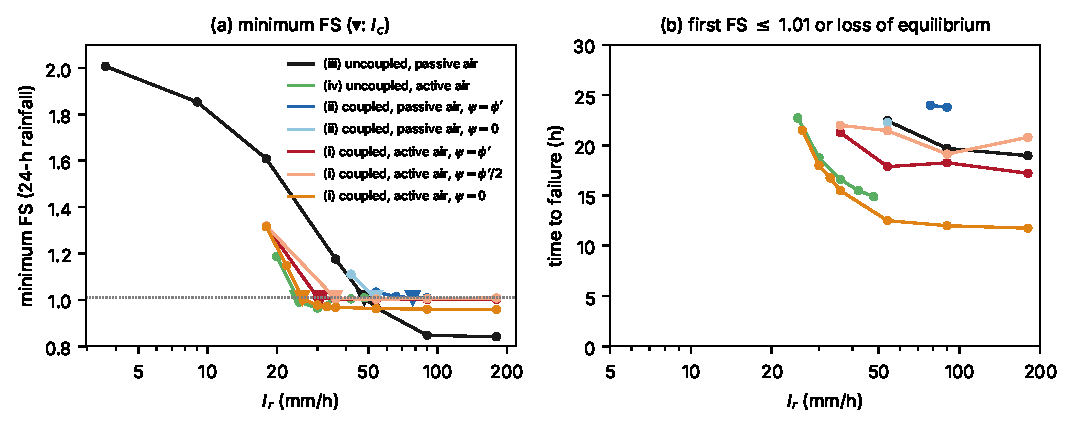
\includegraphics[width=\textwidth]{decomposicao.pdf}
\caption{Soil $f_{50}$, $\alpha=45^\circ$, 24-h rainfalls. (a) Minimum FS against the rainfall intensity in the
four models ($\blacktriangledown$: critical intensity, FS $=1.01$). (b) Time to failure: first instant with FS
$\le1.01$, or loss of equilibrium of the coupled transient with $\psi=0$.}\label{fig:decomp}
\end{figure}

\begin{table}[htbp]
\centering\footnotesize\setlength{\tabcolsep}{4pt}
\caption{Critical intensity ($k_s=36\mmh$) and time to failure of the reference slope. Bracket: computed intensities
on each side of $\Ic$ (FS $\le1.01$); the column FS $\le1.02$ gives $\Ic$ with that threshold. Time to failure: first
instant with FS $\le1.01$; --: no failure; blank: not computed. $^\dagger$Loss of equilibrium of the coupled
transient.}\label{tab:decomp}
\begin{tabular}{lcccccccc}
\toprule
model & $I_c$ & bracket & $I_c/k_s$ & $I_c$ & \multicolumn{4}{c}{time to failure (h) for $I_r$ (mm/h) $=$}\\
 & (mm/h) & (mm/h) & & FS $\le1.02$ & 36 & 48 & 54 & 90\\
\midrule
(iii) uncoupled, passive air & 48 & 48--54 & 1.33 & 47 & -- & -- & 22.4 & 19.7\\
(iv) uncoupled, active air & 25 & 20--25 & 0.69 & 25 & 16.6 & 14.9 &  & \\
(ii) coupled, passive, $\psi=\phi'$ & 78 & 66--78 & 2.16 & 62 &  &  & -- & \\
(ii) coupled, passive, $\psi=0$ & 53 & 42--54 & 1.49 & 52 &  &  & 22.2$^\dagger$ & \\
(i) coupled, active, $\psi=\phi'$ & 31 & 30--36 & 0.86 & 30 & 21.3 &  & 17.9 & 18.3\\
(i) coupled, active, $\psi=\phi'/2$ & 36 & 18--36 & 0.99 & 35 & 22.0 &  & 21.5 & 19.1\\
(i) coupled, active, $\psi=0$ & 26 & 22--26 & 0.72 & 26 & 15.5$^\dagger$ &  & 12.5$^\dagger$ & 12.0$^\dagger$\\
\bottomrule
\end{tabular}

\end{table}

The four models separate the two hypotheses (Table~\ref{tab:decomp}).
\begin{itemize}
\item \emph{The air lowers the critical intensity by about half}: on a rigid skeleton from 48 to 25~mm/h (passive and
active air, models iii and iv); in the coupled models from 53 to 26~mm/h without dilatancy and from 78 to 31~mm/h
with $\psi=\phi'$ (from 62 to 30~mm/h with the threshold 1.02).
\item \emph{The coupling raises it}: by 4--10\% without dilatancy (from 25 to 26~mm/h with active air, from 48 to
53~mm/h with passive air) and by 24--63\% with associated dilatancy (to 31 and 78~mm/h). The deformation of the
skeleton during the wetting, elastic swelling as the effective stress decreases and plastic dilation in the shear
zone, opens pore space and lowers the pore pressures.
\end{itemize}
The two simplifications of the usual model thus have opposite effects: neglecting the deformation is conservative,
neglecting the air is not, and the air dominates. A two-phase flow analysis on a rigid skeleton, model (iv), recovers
the bias: its critical intensity, 25~mm/h, is 4\% below that of the complete model without dilatancy and 20\% below
that with associated dilatancy, and its time to failure with 36~mm/h, 16.6~h, lies between those of the complete model
with $\psi=0$ (15.5~h) and with $\psi=\phi'$ (21.3~h).

The coupled models with an associated flow rule approach one from above (1.000--1.014 for $I_r\ge\Ic$), so their
critical intensity depends on the threshold. With FS $\le1.02$ instead of 1.01 the critical intensities change by
less than 1~mm/h, except that of model (ii) with $\psi=\phi'$, whose minimum FS is 1.033, 1.014 and 1.010 with 54, 66
and 78~mm/h: $\Ic=62$ instead of 78~mm/h. In this model the slope sits in limit equilibrium over a wide range of
intensities, with plastic deformation but without loss of equilibrium.
